% LaTeX.tex
% Template for PROCEEDINGS PAPER of the 28th ABCM International Congress of Mechanical Engineering
% COBEM 2025
% Based on the templates of COBEM2015, COBEM2017, COBEM2019, COBEM2021 and COBEM2023

\documentclass[10pt,fleqn,a4paper,twoside]{article}
\usepackage{abcm}
% \def\shortauthor{F. Author, S. Author and T. Author (update this heading accordingly)}
\def\shortauthor{Rezende, E., Vedovotto, J., Lobato, F., Serfaty, R.}
\def\shorttitle{Signed Log-Uniform Initialization: Extending Logarithmic Sampling to Negative Domains in Evolutionary Optimization}

\begin{document}
\fphead
\hspace*{-2.5mm}\begin{tabular}{||p{\textwidth}}
\begin{center}
\vspace{-4mm}
\title{COB-2025-2080 \\
SIGNED LOG-UNIFORM INITIALIZATION: EXTENDING LOGARITHMIC SAMPLING TO NEGATIVE DOMAINS IN EVOLUTIONARY OPTIMIZATION}
\end{center}
\authors{Estevan Bonadio Augusto Rezende} \\
\authors{João Marcelo Vedovotto} \\
\authors{Fran Sérgio Lobato} \\
\authors{Ricardo Serfaty} \\
\institution{MFLab - Fluid Mechanics Laboratory, Federal University of Uberlândia - UFU - Santa Mônica, Av. João Naves de Ávila , 2121. CEP: 38400-902. Uberlândia - MG - Brazil} \\
\institution{estevan\_rez@ufu.br, vedovotto@ufu.br, fslobato@ufu.br, rserfaty@petrobras.com.br} \\
\\
% The abstract should describe the objectives, context, and significance of the research, methods, results
%, and main conclusions of the paper in about 300 words. It should not include formulas or references to a bibliography. It must be written in only one paragraph.
\abstract{\textbf{Abstract.} A novel method called Virtual Optimization for flame representation in CFD flows has been developed for performance gains when solving reactive flows. 
For this methodology, the correct representation of both temperature and laminar flame speed is achieved. In the the creation process of this methodology, an optimization of a 16-variable problem is required,
of which both polynomial and exponentiation black box configuration are addressed, a coupled thermodynamic representation of heat capacity using JANAF polynomials for a virtual species and the 
use of Arrhenius kinetic parameters with fractional orders for their reaction rates are needed for the full representation. This scheme requires a variable search space composed of many orders
of magnitude with both positive and negative values in a highly non-linear and stiff system. The representation of all orders of magnitude and signs of each variable is an important key point of
the analysis, the use of log uniform distribution would be beneficial, but since it doesn't handle negative values, it would require to double every variable that can also have negative values,
to prevent this increased complexity, a signed version of the log uniform distribution is proposed. By doubling the range of the variable domain and assigning each half to represent the same
value with different signs, each order of magnitude is represented in both sign and value. A comparison is made between linear, log-uniform, and signed log-uniform variable initialization, 
the results provide positive statistical backing for a gain in performance from the use of the new signed log-uniform distribution in comparison to both the unaltered log-uniform distribution 
and linear uniform distribution.}\\
\\
\keywords{\textbf{Keywords:} Evolutionary Optimization, Search Space Exploration, Combustion Process, Logarithmic Sampling, Mixed-Sign Variables.}\\
\end{tabular}

\section{INTRODUCTION}
Industrial-scale combustion processes have been a major focus of research in the past few decades, as there is a growing need to reduce their pollutant emissions. To fully and accurately simulate these processes,
a CFD reactive flow simulation may need to be solved; however, the extremely high computational cost associated with the full analysis may be unachievable with present methods. Because of that,~\citet{Cailler2020} developed a novel method for the reduction of combustion mechanism complexity, to correctly use this new methodology the intermediate virtual species and both Arrhenius 
like reactions for a methane (CH4) 1D flame and its JANAF polynomial coefficients must be optimized. The main focus of the optimization variables is the JANAF coefficients that have to span many orders of magnitude and both positive and negative values, while also having other variables that can have optimized values in a range composed of many decades.
Since the stepping of optimization methods usually involve additive operations, and not multiplicative operations, there can be an underrepresentation of these orders of magnitude; therefore, the use of 
a log-uniform distribution is encouraged~\citep{Bergstra2012}.

The log-uniform distribution requires that the optimization variables be strictly positive and non-zero, this requirement can be overcome by assigning another optimization variable
to represent the sign of the variable, using boolean or integer values to represent positive or negative sign, or even using a range [-1, 1] by passing it through the mathematical sign function, 
although mathematically the same, some optimization methods may not support all of these options, so the user may need to strictly adopt any one of these. The obvious downside is that, for each
log-uniform variable that is not strictly positive, there needs to be a doubling of the number of each of these variables, this may cause many side effects such as: slower convergence, higher 
resource consumption, reference directions or tournament pressure focusing on sign variables without any objective function improvement at evaluation, etc.

As a way to counteract the downside of doubling the number of search space variables, an extension of the log-uniform distribution is proposed. By doubling the search space of a single variable in 
a symmetric manner and defining that the first half corresponds to negative numbers and the second half corresponds to the positive numbers, a single variable can be utilized for both positive and
negative values, while also representing equally all orders of magnitudes. The downsides now only being the inability to represent zero values and the discontinuity between the lowest
represented values. 

The comparison between both methods are made first by establishing a base case, which will use a linear distribution scheme (LIN) with no modification, with 2 optimization variables per physical variable, representing 
its sign and its magnitude, with a discontinuity at zero. The second case is for the log-uniform distribution (LUD) scheme with, also containing 2 optimization variables per physical variable in the same manner as the 
linear case. The last comparison will contemplate the objective of the study, the signed log-uniform distribution (SLUD), which contains a single optimization variable per physical variable. 

For a more direct comparison, a single objective Particle Swarm Optimization (PSO)~\citep{Kennedy1995} routine is used as a first analysis, comparing the number of successful runs, their convergence speed statistics, and the number 
of evaluations to achieve a desired objective variable threshold. The test functions were chosen to compare different aspects of the distributions, 4 in total were chosen, their detailed descriptions 
are described in the text.

\section{METHODOLOGY}

For the currently under development optimization scheme for the virtual chemical optimization, a Non-Dominated Sorting Genetic Algorithm III (NSGA-III)~\citep{Deb2014} is used, but for a comparison of the distributions, a single objective PSO scheme is used, as it is a more straightforward method to analyze the convergence and success of the distributions.
All analyses were done using PYMOO default PSO class with imposed number of individuals~\citep{pymoo} optimization package with RAY~\citep{Ray2018} as a runtime parallelization package, Python version 3.11.4 was used. Each distribution will be evaluated
for each of the test functions and each of the functions will be evaluated with equal: Number of individuals, maximum number of generations, minimum objective function value,
search space size. For the linear case exclusively, the search space will not be in logarithmic space, since it is the baseline case.

\subsection{Distributions}
The initialization of the PSO class is made through the Latin Hypercube Sampling method (LHS)~\citep{McKay1979}, so every stratum of the search space is equally represented, in the linear case this is enough, but for both the 
LUD and SLUD methods the search space must be transferred to the logarithm space before sampling. To make the comparisons more directly comparable, the LIN distribution will have 2 variables, one for sign and another for 
magnitude, the same as LUD. Since the variable space spans many orders of magnitude, the linear LHS sampling makes the distribution become heavily right skewed, as the number of orders increases. This serves
as the baseline case. For this section, an example for physical space exploration of $[-10^3; -10^{-1}] \cup [10^{-1}; 10^{3}] $ will be used.

For the LUD and SLUD cases, the logarithm base 10 of the vector comprising the lower bound (lb) and the upper bound (ub) is taken before the LHS is applied. This ensures each decade is represented by a number with additive properties
(e.g. $[{lb, ub}] \;=\; log_{10}([10^{-1}, 10^{3}])\;=\; [-1,3]$), this makes the distribution be uniform in the logarithm, correctly representing each decade per strata. Equation~(\ref{Eq:lud})
exemplifies the use of 2 variables, where $x_{var}$ is the first variable of the individual after LHS from the bounds vector, and $x_{sign}$ is the second variable from a unitary bounds vector equal to 
$[-1, 1]$. The physical value of these variables is $x_{LUD}$.

\begin{equation}
    x_{\mathrm{LUD}}\;=\;   sign(x_{\mathrm{sign}})\cdot 10^{x_{\mathrm{var}}}
    \label{Eq:lud}
\end{equation}

In the case of the SLUD, the range is doubled, so the vector $x=[-1,3]$ is transformed to $x_2=[-2,6]$, the decades from -2 to 2 represent the negative half and the decades from 2 to 6 represent the positive half.
Before transforming to the physical value, the vector is shifted to be symmetric at 0, represented by $x_{2,sym}=[-4,4]$, this is normalized to unity as $x_{unit}=[-1,1]$. This shift and normalization are only numerically relevant, each created
individual will have values spanning the doubled range, but their final unitary sign will define the effective physical sign and value. 

\begin{equation}
    x_{\mathrm{SLUD}}\;=\; sign(x_{\mathrm{unit}}) \cdot lb \cdot  \left(\frac{ub}{lb}\right)^{| x_{\mathrm{unit}}|}
    \label{Eq:slud}
\end{equation}

Equation~(\ref{Eq:slud}) has a natural interpretation, for negative unitary values, the physical value is negative, the same is said for the positive unitary values, recovering positive physical values.
For the exponent, if it is numerically equal to 1, only the upper bound value is retrieved, if the exponent is numerically zero, the lower bound value is retrieved, 
but undefined in sign. As the exponent grows from 0 to 1, the value varies in a manner similar to a power law, linear in the logarithmic space. These properties are recovered only through the use 
of a single variable.

The most significant drawback for LUD and SLUD applications is the inability to represent zero values, since the logarithm of zero
is undefined, this makes so variables that have zero as a valid value cannot be represented. Another drawback
is the discontinuity between the lower and upper bounds with the numerical value of zero being undefined in sign,
this may cause issues in the optimization process, these 2 aspects will not be the focus of this study.



The linear distribution uses a bounds vector equal to $[10^{-1}, 10^{3}]$, while the LUD has a bounds vector equal to $[-1,3]$ and the SLUD bounds vector is $[-2,6]$. Although these values are not 
equal, their representation in physical space is the same if accompanied by their respective sign defining extra variables, the only difference is the uniform distribution property of the linear case, and
the uniform distribution in logarithmic space property of the LUD and SLUD case.

\subsection{Optimization}
For the comparison between these distributions, 3 Python scripts were written, one containing the distribution functions with the optimization algorithm runner, another with all the functions to be 
compared against, and finally a statistical analyser for the created CSV files, in total 4 functions were chosen for evaluation, with 2 of these having a sign-flipped variant where we substituted $x_2$ with $-x_2$ in the objective function. This modification preserves the mathematical properties of the original problem while requiring the optimizer to find a solution with a negative value for $x_2$ instead of a positive one, 
allowing us to test how each distribution method handles optimization with a mixed domain. The optimizations are strictly derivative free. The LIN and LUD cases have double the number of variables compared to the SLUD case, as to
represent the sign of each variable.

\subsubsection{Rosenbrock}
One of the most well known test functions commonly referred to as Rosenbrock, its 2D variant is defined as:

\begin{equation}
    f(x_1, x_2) = 100 \cdot (x_2 - x_1^2)^2 + (1 - x_1)^2
    \label{Eq:rosenbrock}
\end{equation}

The global minimum is at $x^* = [1, 1]$ with $f(x^*) = 0$. The function is non-linear and has a narrow valley around the global minimum, which makes it difficult for optimization algorithms to converge.
As a benchmark starting point, the use of a well known test function is proposed, the Rosenbrock function is a common choice for optimization algorithms, as it has a known global minimum and a well defined shape.

Its lower bound (or the minimum absolute achievable value) is defined as $lb = [10^{-4}, 10^{-4}]$, and the upper bound (or the maximum absolute achievable value) is defined as $ub = [10^{2}, 10^{2}]$.



\subsubsection{Powell Badly Scaled}
The Powell's Badly Scaled Function is proposed as the second evaluation function since it is classified as "badly scaled", The functions are defined as:

\begin{equation}
f_1(x) = 10^4 \cdot x_1 \cdot x_2 -1
\label{Eq:powell1}
\end{equation}
\begin{equation}
f_2(x) = e^{-x_1} + e^{-x_2} - 1.0001 
\label{Eq:powell2}
\end{equation}

Its global minimum is defined as $x^* \approx [1.098, 9.106\cdot10^{-5}]$ with $f(x^*) = (f_1(x^*))^2 + (f_2(x^*))^2 = 0$. For its use in the research, it has been proposed that 
both variables have the same bounds, so a permutation of the variable solution vector is also valid. To compare the use of both positive and negative values in the search space,
2 evaluations will be made, one for the original function, and the second with the terms $x_2$ of the functions being replaced by its negative counterpart, to artificially force a negative 
optimization variable, without changing the final result.

Its lower bound is $lb = [10^{-6}, 10^{-6}]$, while its upper bound is equal to $ub = [10^{2}, 10^{2}]$.


\subsubsection{Brown Badly Scaled}
Another ill-conditioned function used is the Brown Badly Scaled Function, also being non-linear.  The 12-order-of-magnitude difference between the 2 variables in the solution 
vector can exemplify the same aspect seen in the search space for pre-exponential variables of virtual optimized chemistry.

\begin{equation}
f_1(x_1) = x_1 - 10^{6}
\label{Eq:brown1} 
\end{equation}
\begin{equation}
f_2(x_2) = x_2 - 2\cdot 10^{-6}
\label{Eq:brown2}
\end{equation}
\begin{equation}
f_3(x_1,x_2) = x_1 \cdot x_2 - 2
\label{Eq:brown3}
\end{equation}

The global optimum variable vector is $x^* = [1\cdot10^6, 2\cdot10^{ -6} ]$, with global minimum equal to $f(x^*) = (f_1(x^*))^2 + (f_2(x^*))^2 + (f_3(x^*))^2= 0$. Analogous to 
the Powell's function, the permutation of the variable solution vector will also be considered a valid solution. The same double analysis with $x_2$ sign change will be done for the Brown
Badly Scaled function.

The defined lower bound is $lb = [10^{-8}, 10^{-8}]$, while the upper bound is $ub = [10^{8}, 10^{8}]$.


\subsubsection{Poly7: Heat Capacity}
For a more direct comparison of the optimization of the JANAF polynomials, a synthetic test is also proposed. One of the new steps in the analysis of the virtual scheme involves the use of Propane (C3H8) based
fuels, in particular, the heat capacity (Cp) representation in a temperature interval is one of the most important steps to reproduce the flame temperature, as enthalpy terms may be simplified to a 
purely Cp based analysis, but the use of a constant heat capacity term introduces significant errors. This optimization consists on recovering the first 5 polynomial coefficients of the GRI-Mech 3.0
Mechanism~\citep{GRIMech30} C3H8 species in the interval of temperature range $[200, 1000]$ Kelvin. This polynomial is:

\begin{equation}
\frac{Cp(T)}{R} = 0.93355381 +  0.026424579 \cdot T +  6.1059727\cdot10^{-6} \cdot T^2 - 2.1977499\cdot10^{-8} \cdot T^3 + 9.5149253\cdot 10^{-12} \cdot T^4
\label{Eq:poly7}
\end{equation}

Since the universal gas constant is only a scaling term, at evaluation time it is not explicitly used. The evaluation function is composed by the Mean Relative Squared Error metric between the 
evaluation of the original polynomial for a number of sample points in the temperature range, versus the same evaluation of a polynomial composed by 5 coefficients created from the optimization
procedure. The global minimum of the function is achieved when the numerical values of the optimization variables are identical to the original Eq.~(\ref{Eq:poly7}). 

The lower bound for the poly7 function is defined as $lb = [10^{-2}, 10^{-5}, 10^{-8}, 10^{-11}, 10^{-14}]$, the upper bound is $ub = [10^{2}, 10^{-1}, 10^{-4}, 10^{-7}, 10^{-10}]$.

\subsection{OPTIMIZATION PARAMETERS}

In an effort to minimize variations between comparisons, all parameters related to each function evaluation is maintained equal for every distribution utilized. For all optimizations the number of 
individuals is equal to 100, the maximum number of generations to be evaluated is 500 per optimization, the PSO algorithm default initialization sampling is LHS for all cases. An optimization
will end if the maximum number of generations is achieved (unsuccessful run) or if the minimum objective function value is achieved, the latter case is defined as a successful run.

The target minimum objective function for each function in is: $f_{min}(Rosenbrock) = 10^{-8}$, $f_{min}(Powell) = 10^{-10}$, $f_{min}(Brown) = 10^{-10}$, $f_{min}(Poly7) =  10^{-5}$. Each value was chosen based 
on reasonable estimates based on individual testing, in a purely speculative manner, in special, the use of a high objective function value of the polynomial case will be explained
in the latter sections.

\subsection{STATISTICAL ANALYSIS}

For each of the 3 defined distributions, for each of the 6 predefined functions, accounting also the simple change of sign of Powell and Brown functions, a statistical comparison is made.
Totaling 18 sets of data, the mean, median, standard deviation, and quartile ranges for 200 runs will be tallied, composed with their respective success rate percentages and the maximum and minimum 
number of iterations to relative convergence. 

\section{RESULTS}

The authors' own computational resources were utilized, each optimization run was collected in a comma-separated value file (CSV), after all data points are collected, the statistical metrics
are obtained and saved.% A repository with the code and data files is available at the following URL: https://1drv.ms/f/c/91e7db8e6c7d12f6/EjKzfXNKMlpFlEmiOFP49zABeID0Gtyf-foN1tPtdGLlaQ?e=tngYD9.

\subsection{Statistical Results}

The statistical results of each function is presented in each respective table, first the Rosenbrock function represented by Tab.~\ref{Tab:1}:


\begin{table}[H]
\centering
\caption{Statistical results for the Rosenbrock function optimization using different distributions.}
\label{Tab:1}
\begin{tabular}{l|c|c|c|c|c|c|c}
\hline
\textbf{Function} & \textbf{Mean $\pm$ STD} & \textbf{Median} & \textbf{Min} & \textbf{Max} & \textbf{Success Rate (\%)} & \textbf{Q1 Quartile} & \textbf{Q3 Quartile}\\
\hline
Rosen + LIN            & 195.9 $\pm$ 80.8      & 180.0 & 50.0 & 433.0 & 93.0 & 126.8 & 252.3\\
Rosen + LUD            & 166.2 $\pm$ 36.4      & 160.0 & 87.0 & 299.0 & 100.0 & 140.0 & 187.8\\
Rosen + SLUD           & 187.9 $\pm$ 27.7      & 188.0 & 124.0 & 273.0 & 100.0 & 167.3 & 205.0\\
\hline
\end{tabular}
\end{table}

For the Powell function, represented by Tab.~\ref{Tab:2}:

\begin{table}[H]
\centering
\caption{Statistical results for the Powell function optimization using different distributions.}
\label{Tab:2}
\begin{tabular}{l|c|c|c|c|c|c|c}
\hline
\textbf{Function} & \textbf{Mean $\pm$ STD} & \textbf{Median} & \textbf{Min} & \textbf{Max} & \textbf{Success Rate (\%)} & \textbf{Q1 Quartile} & \textbf{Q3 Quartile}\\
\hline
Powell + LIN         & 287.6 $\pm$ 120.6     & 292.0 & 84.0 & 500.0 & 10.5 & 181.0 & 373.5\\
Powell + LUD         & 232.1 $\pm$ 140.2     & 165.5 & 51.0 & 472.0 & 10.0 & 131.5 & 394.8\\
Powell + SLUD        & 193.1 $\pm$ 89.9      & 185.0 & 66.0 & 381.0 & 7.5 & 99.0 & 241.0\\
\hline
\end{tabular}
\end{table}

This Powell function with the sign change is represented by Tab.~\ref{Tab:2b}:

\begin{table}[H]
\centering
\caption{Statistical results for the Powell function with sign change optimization using different distributions.}
\label{Tab:2b}
\begin{tabular}{l|c|c|c|c|c|c|c}
\hline
\textbf{Function} & \textbf{Mean $\pm$ STD} & \textbf{Median} & \textbf{Min} & \textbf{Max} & \textbf{Success Rate (\%)} & \textbf{Q1 Quartile} & \textbf{Q3 Quartile}\\
\hline
Powell + LIN(-)         & 336.7 $\pm$ 104.2     & 375.0 & 177.0 & 500.0 & 11.5 & 228.0 & 406.0\\
Powell + LUD(-)         & 244.3 $\pm$ 122.8     & 238.0 & 75.0 & 468.0 & 7.5 & 120.0 & 346.0\\
Powell + SLUD(-)        & 248.9 $\pm$ 129.1     & 258.0 & 60.0 & 494.0 & 9.5 & 102.0 & 337.0\\
\hline
\end{tabular}
\end{table}

For the Brown function, represented by Tab.~\ref{Tab:3}:

\begin{table}[H]
\centering
\caption{Statistical results for the Brown function optimization using different distributions.}
\label{Tab:3}
\begin{tabular}{l|c|c|c|c|c|c|c}
\hline
\textbf{Function} & \textbf{Mean $\pm$ STD} & \textbf{Median} & \textbf{Min} & \textbf{Max} & \textbf{Success Rate (\%)} & \textbf{Q1 Quartile} & \textbf{Q3 Quartile}\\
\hline
Brown + LIN          & 154.2 $\pm$ 56.4      & 134.5 & 103.0 & 474.0 & 66.0 & 120.0 & 164.5\\
Brown + LUD          & 117.4 $\pm$ 35.4      & 111.0 & 86.0 & 438.0 & 90.0 & 104.0 & 119.0\\
Brown + SLUD         & 111.0 $\pm$ 6.3       & 110.5 & 95.0 & 125.0 & 100.0 & 107.0 & 116.0\\
\hline
\end{tabular}
\end{table}

For the Brown function with the sign change, represented by Tab.~\ref{Tab:3b}:

\begin{table}[H]
\centering
\caption{Statistical results for the Brown function with sign change optimization using different distributions.}
\label{Tab:3b}
\begin{tabular}{l|c|c|c|c|c|c|c}
\hline
\textbf{Function} & \textbf{Mean $\pm$ STD} & \textbf{Median} & \textbf{Min} & \textbf{Max} & \textbf{Success Rate (\%)} & \textbf{Q1 Quartile} & \textbf{Q3 Quartile}\\
\hline
Brown + LIN(-)          & 163.1 $\pm$ 72.6      & 138.5 & 100.0 & 490.0 & 57.0 & 122.0 & 170.8\\
Brown + LUD(-)          & 124.4 $\pm$ 55.0      & 111.0 & 83.0 & 499.0 & 84.5 & 106.0 & 119.5\\
Brown + SLUD(-)         & 111.8 $\pm$ 6.2       & 112.0 & 96.0 & 129.0 & 100.0 & 107.3 & 116.0\\
\hline
\end{tabular}
\end{table}


For the Poly7 function, represented by Tab.~\ref{Tab:4}:

\begin{table}[H]
\centering
\caption{Statistical results for the Poly7 function optimization using different distributions.}
\label{Tab:4}
\begin{tabular}{l|c|c|c|c|c|c|c}
\hline
\textbf{Function} & \textbf{Mean $\pm$ STD} & \textbf{Median} & \textbf{Min} & \textbf{Max} & \textbf{Success Rate (\%)} & \textbf{Q1 Quartile} & \textbf{Q3 Quartile}\\
\hline
Poly7 + LIN          & 122.5 $\pm$ 99.6      & 97.0 & 29.0 & 392.0 & 7.5 & 45.0 & 151.0\\
Poly7 + LUD          & 122.1 $\pm$ 117.0     & 68.5 & 18.0 & 497.0 & 52.0 & 31.0 & 202.8\\
Poly7 + SLUD         & 148.0 $\pm$ 132.5     & 77.0 & 13.0 & 497.0 & 55.0 & 36.0 & 246.3\\
\hline
\end{tabular}
\end{table}


\subsection{Discussion}

The Rosenbrock function statistic show that both SLUD and LUD have a higher success rate than the linear distribution, with the SLUD having a slightly higher mean and median, but with a lower standard deviation, 
this shows that the log-uniform distribution method is marginally more effective than the linear distribution for this case. The SLUD has a higher mean and median than the LUD, but with a lower standard deviation, 
LUD appears to be more effective than the SLUD for this case, but care must be taken since the number of variables is not the same, this may show that SLUD is a viable option, but not necessarily better than LUD.


By reviewing both Tab.~\ref{Tab:2} and Tab.~\ref{Tab:2b} the linear case has a marginally higher success rate, but a higher mean, min and 
quartile results, the results from the LUD and SLUD are very similar, with no noteworthy differences, this case may indicate that
the use of a single variable for both positive and negative values may not interfere with the optimization process.


From the data gathered in Tab.~\ref{Tab:3} and Tab.~\ref{Tab:3b}, both linear evaluations have a lower success rate than the log-uniform and signed log-uniform distributions, with the SLUD having a
lower mean and standard deviation than the LUD and a higher success rate, this shows that the SLUD is more effective than the LUD for this case. The discrepancy between the standard deviations
may indicate that the SLUD is more effective than the LUD and LIN, especially by taking into consideration the Max number of iterations, is nearly a fourth of the LUD and LIN. However, the
quartiles show that it may be related to a rogue individual that was not able to converge.

In the case of the Poly7 function, the SLUD has a higher mean, standard deviation and median than the LUD, but a slightly higher success rate. The most important aspect of this function is that the
success rate is very low for the linear distribution, with only 7.5\% of the runs being successful, while the LUD and SLUD have a success rate of 52\% and 55\% respectively, reaffirming the importance
of the logarithmic sampling for this case.

The Poly7 function is a mock test function, so the objective function value is not as important as the success rate.
A random sample of the converged polynomial coefficients is shown in Fig.~\ref{Fig:1}, where the black continuous line represents the original polynomial and the red dashed line
represents the polynomial created by the optimization procedure $Cp_{opt} \approx 2.786\cdot10^{-1} + 3.230\cdot10^{-2} -1.176\cdot10^{-5} + 6.885\cdot10^{-11} + 4.474\cdot10^{-14}$, by comparing 
this with the original polynomial coefficients, there is a huge discrepancy between the values, but by comparing the plotted curves, it is seen how closely the converged polynomial matches the 
original shape in the temperature range of interest. This fact is the most important aspect of the thermal properties optimization, and a novel detail to the original posed problem, since, between optimizations runs,
a polynomial with a different set of coefficients could, and usually would, be generated.

\begin{figure}[h!]
\centering
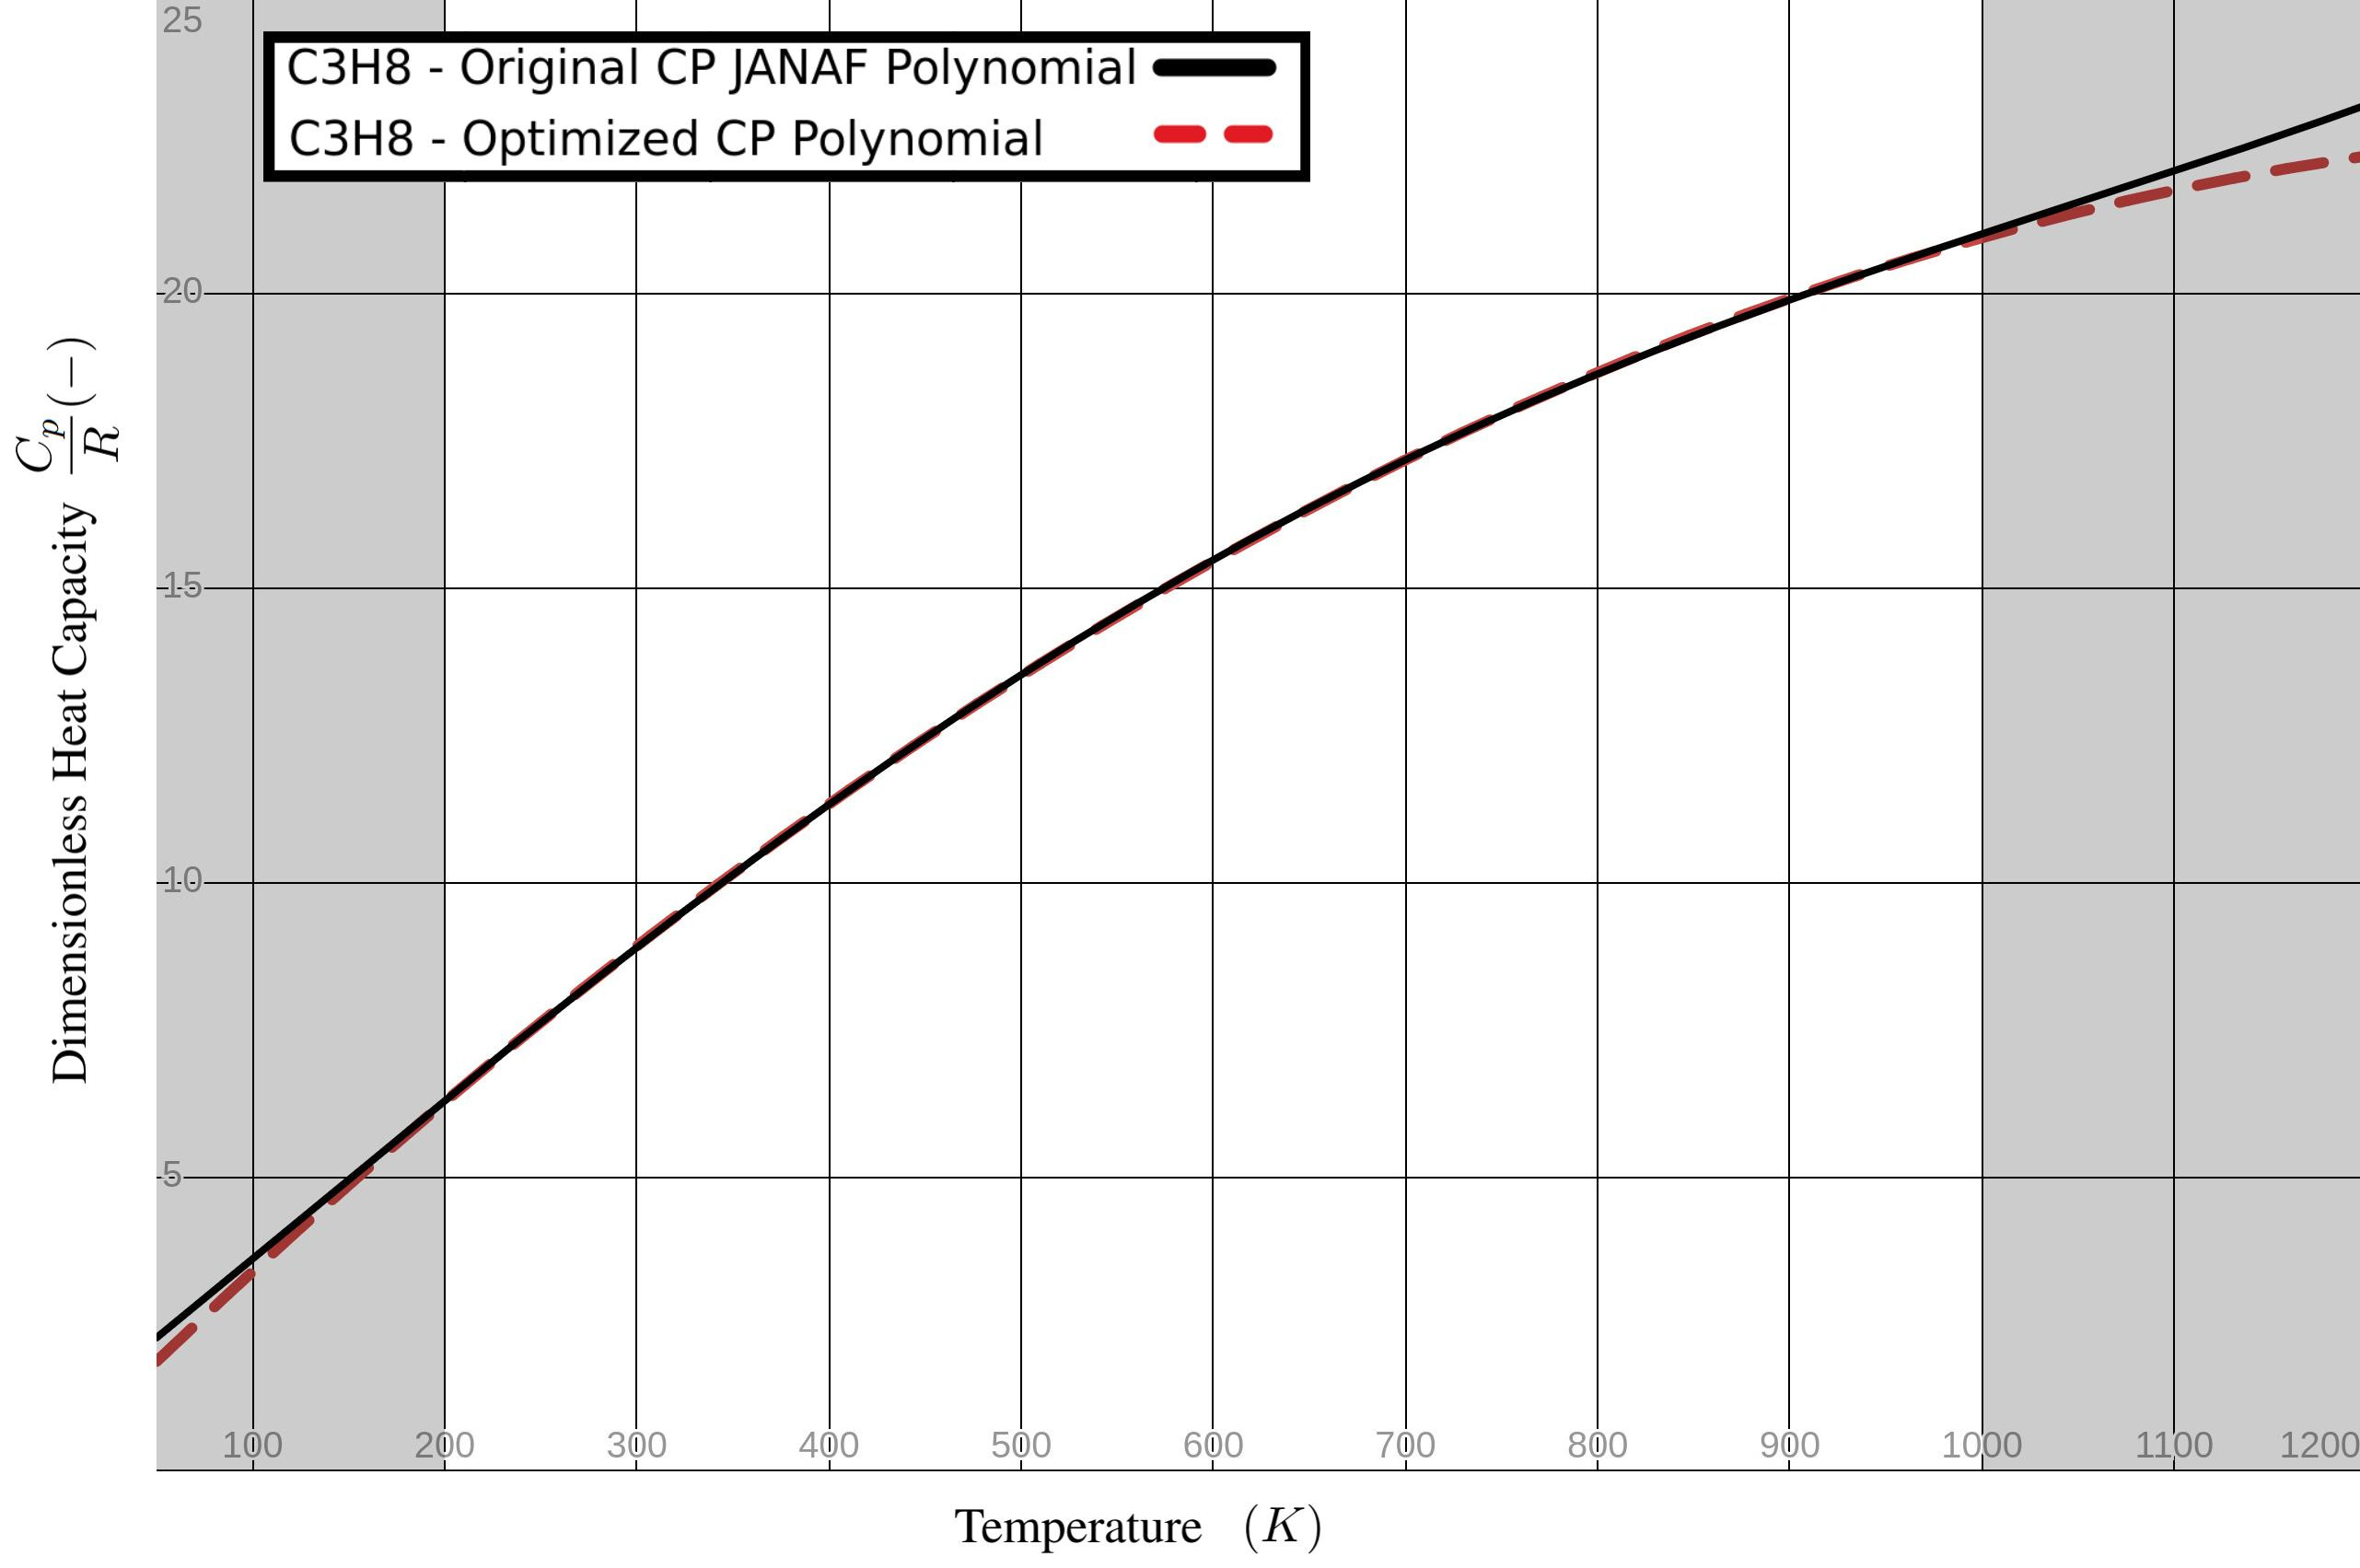
\includegraphics[angle=0, width=17cm]{C3H8.jpeg}
\caption{Comparison between the C3H8 temperature bounded $\frac{C_p}{R}$ (black continuous line) and the randomly sampled converged polynomial (red dashed line). Shaded region (left and right) indicate the temperatures outside the calibrated range lower temperature interval.}
\label{Fig:1}
\end{figure}

\section{CONCLUSION}

The comparison between the linear, log-uniform, and signed log-uniform distributions shows that the use of logarithmic based distributions is very beneficial for the optimization of functions with variables that span many orders of magnitude, 
the decrease in the number of iterations needed for convergence and the increase in the success rate of the optimization runs demonstrate well the net positives of log-uniform distribution.
There were no cases in the evaluated functions where the linear distribution was explicitly more effective than both counterpart, the SLUD and LUD distributions, even though the premise of utilizing a single
variable for both positive and negative values on SLUD may at first seem to be an advantage, the results show that the LUD is still slightly more effective than the SLUD, but the difference
may not be significant enough to warrant the use of 2 variables for each physical variable depending on a case by case basis.

A couple points of interest may be brought up from the analysis, the use of equal seeds for each data gathering loop may have caused a bias in the results, as the same individuals were used for each distribution,
but that could also be a point of interest, as these equal individuals were evaluated with different distributions, the similarity of the results from the sign-changed Powell and Brown functions should be investigated further. Another point may be the low number of samples, an increase from 200 runs to a more statistically significant number could
generate clearer results, but the time needed to run the optimizations would increase significantly, so a balance between time and statistical significance was made. 

The signed log-uniform distribution is a novel method for the representation of both positive and negative values in a logarithmic space, while also being able to represent all orders of magnitude in a
simple manner, with minimal increase in complexity, user input, and computational resources. One could even argue that these positive traits could be even more beneficial in a multi-objective optimization scheme, as the number of variables would be halved, and the search space would be more compact, allowing for a more efficient exploration of the search space.

Future works will focus on the use of the signed log-uniform distribution in a multi-objective optimization scheme, as well as the use of other optimization algorithms, in particular for the NSGA-III,
since the convergence of temperature, laminar flame speed, and heat release rate are all important aspects of the virtual optimization scheme.

\section{ACKNOWLEDGEMENTS}

This work was funded directly by PETROBRAS as part of the virtual optimization scheme research project. We would also like to extend the thanks to FAPEMIG for helping fund the transport arrangements and 
other costs related to the participation of the authors and research fellows from MFLab for COBEM 2025.

\section{REFERENCES} 
\label{Sec:references}

\bibliographystyle{abcm}
\renewcommand{\refname}{}
\bibliography{bibfile}

\section{RESPONSIBILITY NOTICE}
The authors are solely responsible for the printed material included in this paper.

\end{document}
